\tikzstyle{startstop} = [rectangle, rounded corners, minimum width=10cm, minimum height=1.5cm,text centered, draw=black, fill=green!20]
\begin{center}
	\begin{tikzpicture}
		\node (start) [startstop] {\bfseries \text{ÔN TẬP: GIA TỐC - CHUYỂN ĐỘNG THẲNG BIẾN ĐỔI ĐỀU}};
	\end{tikzpicture}
\end{center}
\setcounter{section}{0}
\Opensolutionfile{ans}[ans/G10TUAN4-TN]
% ===================================================================
\begin{ex}
	Gia tốc là đại lượng
	\choice
	{vô hướng, đặc trưng cho sự biến thiên nhanh hay chậm của chuyển động}
	{vô hướng, đặc trưng cho tính không đổi của vận tốc}
	{vector, đặc trưng cho sự biến thiên nhanh hay chậm của chuyển động}
	{\True vector, đặc trưng cho sự biến thiên nhanh hay chậm của vận tốc}
	\loigiai{}
\end{ex}
% ===================================================================
\begin{ex}
	Chọn ý \textbf{sai}. Chuyển động thẳng nhanh dần đều có
	\choice
	{\True vector gia tốc ngược chiều vector vận tốc}
	{vận tốc tức thời là hàm số bậc nhất theo thời gian}
	{toạ độ là hàm số bậc hai theo thời gian}
	{gia tốc không đổi theo thời gian}
	\loigiai{}
\end{ex}
% ===================================================================
\begin{ex}
	Một xe máy đang đứng yên, sau đó khởi động và bắt đầu tăng tốc. Nếu chọn chiều dương cùng chiều chuyển động của xe, nhận xét nào sau đây là \textbf{đúng}? 
	\choice
	{$a<0$, $v<0$}
	{$a>0$, $v<0$}
	{\True $a>0$, $v>0$}
	{$a<0$, $v>0$}
	\loigiai{}
\end{ex}

% ===================================================================
\begin{ex}
Công thức tính quãng đường đi được của vật chuyển động thẳng nhanh dần đều là	
	\choice
	{\True $s=v_0t+\frac{1}{2}at^2$ ($a$ và $v_0$ cùng dấu)}
	{$s=v_0t+\frac{1}{2}at^2$ ($a$ và $v_0$ trái dấu)}
	{$s=at+\frac{1}{2}v_0t^2$ ($a$ và $v_0$ cùng dấu)}
	{$s=at+\frac{1}{2}v_0t^2$ ($a$ và $v_0$ trái dấu)}
	\loigiai{}
\end{ex}
% ===================================================================
\begin{ex}
Tàu hoả đang chuyển động thẳng với tốc độ $\SI{60}{\kilo\meter/\hour}$ thì bị hãm phanh, chuyển động chậm dần đều. Sau khi đi thêm được $\SI{450}{\meter}$ thì tốc độ của tàu chỉ còn $\SI{15}{\kilo\meter/\hour}$. Quãng đường tàu còn đi thêm được đến khi dừng hẳn là	
	\choice
	{$\SI{60}{\meter}$}
	{$\SI{45}{\meter}$}
	{$\SI{15}{\meter}$}
	{\True $\SI{30}{\meter}$}
	\loigiai{}
\end{ex}
% ===================================================================
\begin{ex}
Một ô tô chuyển động chậm dần đều. Sau $\SI{10}{\second}$, tốc độ của ô tô giảm từ $\SI{6}{\meter/\second}$ còn $\SI{4}{\meter/\second}$. Quãng đường ô tô đi được trong khoảng thời gian $\SI{10}{\second}$ đó là	
	\choice
	{$\SI{70}{\meter}$}
	{$\SI{50}{\meter}$}
	{$\SI{40}{\meter}$}
	{\True $\SI{100}{\meter}$}
	\loigiai{}
\end{ex}
% ===================================================================
\begin{ex}
Một ô tô đang chuyển động với tốc độ $\SI{10}{\meter/\second}$ thì bắt đầu tăng tốc, chuyển động nhanh dần đều. Sau $\SI{20}{\second}$ kể từ khi tăng tốc, ô tô đạt tốc độ $\SI{14}{\meter/\second}$. Sau $\SI{50}{\second}$ kể từ lúc tăng tốc, gia tốc và vận tốc của ô tô lần lượt là	
	\choice
	{$\SI{0.2}{\meter/\second^2}$ và $\SI{18}{\meter/\second}$}
	{\True $\SI{0.2}{\meter/\second^2}$ và $\SI{20}{\meter/\second}$}
	{$\SI{0.4}{\meter/\second^2}$ và $\SI{38}{\meter/\second}$}
	{$\SI{0.1}{\meter/\second^2}$ và $\SI{28}{\meter/\second}$}
	\loigiai{}
\end{ex}
% ===================================================================
\begin{ex}
	Một vật chuyển động thẳng có quãng đường đi trong một giai đoạn phụ thuộc thời gian dạng $s=-t^2+3t$ ($s$ đo bằng $\si{\meter}$; $t$ đo bằng giây). Biểu thức vận tốc của vật theo thời gian trong giai đoạn này được xác định bởi
	\choice
	{$v=3+2t$}
	{$v=2-3t$}
	{$v=3-t$}
	{\True $v=3-2t$}
	\loigiai{}
\end{ex}

% ===================================================================
\begin{ex}
Một xe chuyển động trên đường thẳng với biểu thức toạ độ phụ thuộc thời gian: $x=0,4t^2+2t+1$ ($x$ tính bằng $\si{\meter}$; $t$ tính bằng $\si{\second}$). Vận tốc của xe tại thời điểm $t=\SI{5}{\second}$ là
	\choice
	{$\SI{10.4}{\meter/\second}$}
	{$\SI{4.0}{\meter/\second}$}
	{$\SI{5.0}{\meter/\second}$}
	{\True $\SI{6.0}{\meter/\second}$}
	\loigiai{}
\end{ex}

% ===================================================================
\begin{ex}
Một ô tô đang chạy với tốc độ $\SI{10}{\meter/\second}$ trên đoạn đường thẳng thì người lái xe tăng ga và ô tô chuyển động nhanh dần đều. Sau một khoảng thời gian, ô tô đạt tốc độ $\SI{15}{\meter/\second}$. Tốc độ trung bình của ô tô trong khoảng thời gian đó là	
	\choice
	{\True $\SI{12.5}{\meter/\second}$}
	{$\SI{9.5}{\meter/\second}$}
	{$\SI{21}{\meter/\second}$}
	{$\SI{2.5}{\meter/\second}$}
	\loigiai{}
\end{ex}
% ===================================================================
\begin{ex}
	Một vật chuyển động thẳng có phương trình toạ độ $x=20t^2+40t+6$ ($\si{\centi\meter}$; $\si{\second}$). Gia tốc và tính chất chuyển động của vật là
	\choice
	{\True $\SI{40}{\centi\meter/\second^2}$; vật chuyển động nhanh dần đều}
	{$\SI{40}{\centi\meter/\second^2}$; vật chuyển động chậm dần đều}
	{$\SI{20}{\centi\meter/\second^2}$; vật chuyển động nhanh dần đều}
	{$\SI{20}{\centi\meter/\second^2}$; vật chuyển động chậm dần đều}
	\loigiai{}
\end{ex}
% ===================================================================
\begin{ex}
	Lúc $\SI{1}{\hour}$, một xe máy qua A với tốc độ $\SI{10}{\meter/\second}$, chuyển động nhanh dần đều với gia tốc $\SI{1}{\meter/\second^2}$ đuổi theo một xe đạp đang chuyển động nhanh dần đều qua B với tốc độ đầu là $\SI{2}{\meter/\second}$ và với gia tốc $\SI{0.5}{\meter/\second^2}$. Sau $\SI{20}{\second}$ thì xe máy đuổi kịp xe đạp. Khoảng cách AB là
	\choice
	{$\SI{360}{\meter}$}
	{$\SI{160}{\meter}$}
	{$\SI{165}{\meter}$}
	{\True $\SI{260}{\meter}$}
	\loigiai{}
\end{ex}
% ===================================================================
\begin{ex}
	Hai người đi xe đạp khởi hành cùng 1 lúc và đi ngược chiều nhau. Người thứ nhất có tốc độ đầu là $\SI{18}{\kilo\meter/\hour}$ và chuyển động chậm dần đều với gia tốc có độ lớn $\SI{20}{\centi\meter/\second^2}$. Người thứ 2 có tốc độ đầu là $\SI{5.4}{\kilo\meter/\hour}$ và chuyển động nhanh dần đều với gia tốc có độ lớn $\SI{0.2}{\meter/\second^2}$. Khoảng cách ban đầu giữa hai người là $\SI{130}{\meter}$. Sau bao lâu 2 người sẽ gặp nhau và gặp nhau ở vị trí nào?
	\choice
	{\True Sau $\SI{20}{\second}$, cách A đoạn $\SI{60}{\kilo\meter}$}
	{Sau $\SI{17.5}{\second}$, cách A đoạn $\SI{56.9}{\kilo\meter}$}
	{Sau $\SI{20}{\second}$, cách B đoạn $\SI{60}{\kilo\meter}$}
	{Sau $\SI{17.5}{\second}$, cách B đoạn $\SI{56.9}{\kilo\meter}$}
	\loigiai{}
\end{ex}
% ===================================================================
\begin{ex}
	Một vật chuyển động trên đường thẳng có đồ thị vận tốc - thời gian như hình vẽ. Quãng đường vật đi được trong $\SI{400}{\second}$ là 
	\begin{center}
		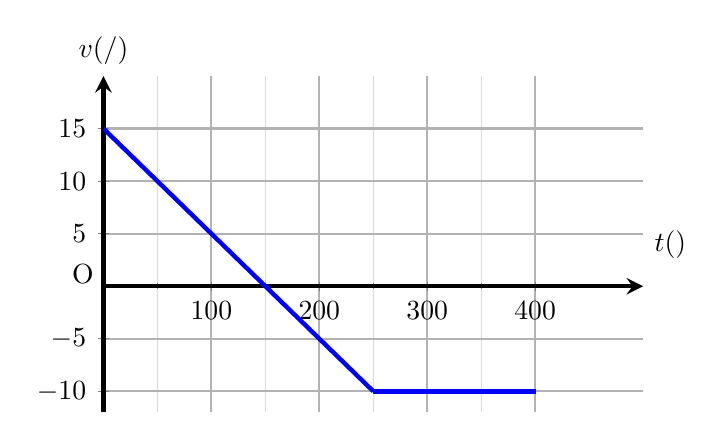
\begin{tikzpicture}  
			\begin{axis}[  ultra thick,yscale=0.75,
				xmin=0,  
				xmax=500,  
				xtick={0,100,...,400},
				ytick={-10,-5,...,15},
				minor x tick num=1,
				minor y tick num=0,
				ymin=-12,  
				ymax=20, 
				samples=300,
				axis lines=center, 
				grid style={step=1, line width =0.4pt, color=gray!30!white},
				grid=both,
				major grid style={line width=0.8pt,gray!60!white},
				xlabel=$\xsi{t}{\left(\si{\second}\right)}$, 		ylabel=$\xsi{v}{\left(\si{\meter/\second}\right)}$,
				every axis y label/.style={at=(current axis.above origin),anchor=south},  
				every axis x label/.style={at=(current axis.right of origin),anchor=west},  ]
				\addplot [ultra thick, blue, smooth, domain=0:250] {15-0.1*x};  
				\addplot [ultra thick, blue, smooth, domain=250:400] {-10};
			 
			\end{axis}  
			\node[below left] at (0,2) {O};
		\end{tikzpicture}
	\end{center}
	\choice
	{$\SI{4625}{\meter}$}
	{\True $\SI{3125}{\meter}$}
	{$\SI{4250}{\meter}$}
	{$\SI{2625}{\meter}$}
	\loigiai{}
\end{ex}
% ===================================================================
\begin{ex}
Một vật chuyển động thẳng có đồ thị vận tốc theo thời gian như hình vẽ. Quãng đường vật đi được trong giai đoạn chuyển động chậm dần đều là	
\begin{center}
	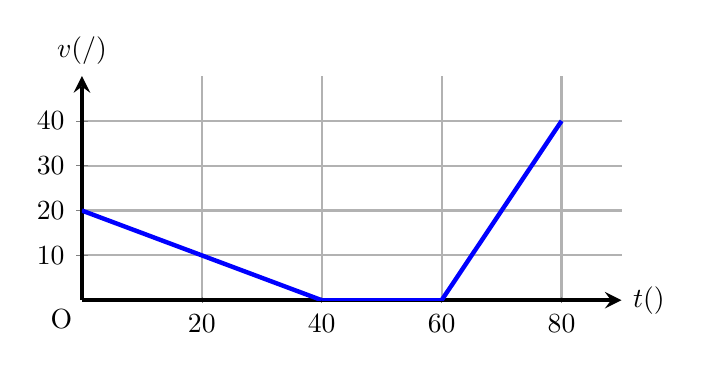
\begin{tikzpicture}  
		\begin{axis}[  ultra thick,yscale=0.5,
			xmin=0,  
			xmax=90,  
			xtick={0,20,...,80},
			ytick={0,10,...,40},
			minor x tick num=0,
			minor y tick num=0,
			ymin=0,  
			ymax=50, 
			samples=300,
			axis lines=center, 
			grid style={step=1, line width =0.4pt, color=gray!30!white},
			grid=both,
			major grid style={line width=0.8pt,gray!60!white},
			xlabel=$\xsi{t}{\left(\si{\second}\right)}$, 		ylabel=$\xsi{v}{\left(\si{\meter/\second}\right)}$,
			every axis y label/.style={at=(current axis.above origin),anchor=south},  
			every axis x label/.style={at=(current axis.right of origin),anchor=west},  ]
			\addplot [ultra thick, blue, smooth, domain=0:40] {20-0.5*x};  
			\addplot [ultra thick, blue, smooth, domain=40:60] {0};
			\addplot [ultra thick, blue, smooth, domain=60:80] {2*(x-60)};
			
		\end{axis}  
	\node[below left] at (0,0) {O}; 
	\end{tikzpicture}
\end{center}
	\choice
	{$\SI{600}{\meter}$}
	{$\SI{800}{\meter}$}
	{$\SI{200}{\meter}$}
	{\True $\SI{400}{\meter}$}
	\loigiai{}
\end{ex}







\Closesolutionfile{ans}
\begin{center}
	\textbf{--- HẾT ---}
\end{center}